%-----------------------------------------------------------------------------%
\chapter{\babTiga}
%-----------------------------------------------------------------------------%

%-----------------------------------------------------------------------------%
\section{Alur Penelitian}
%-----------------------------------------------------------------------------%
Dalam suatu penelitian, terdapat urutan tahapan yang perlu dilakukan. Alur penelitian ini mengandung seluruh langkah yang harus ditempuh, mulai dari fase perancangan hingga tahap akhir penelitian.
 \begin{figure}
	\begin{center}
		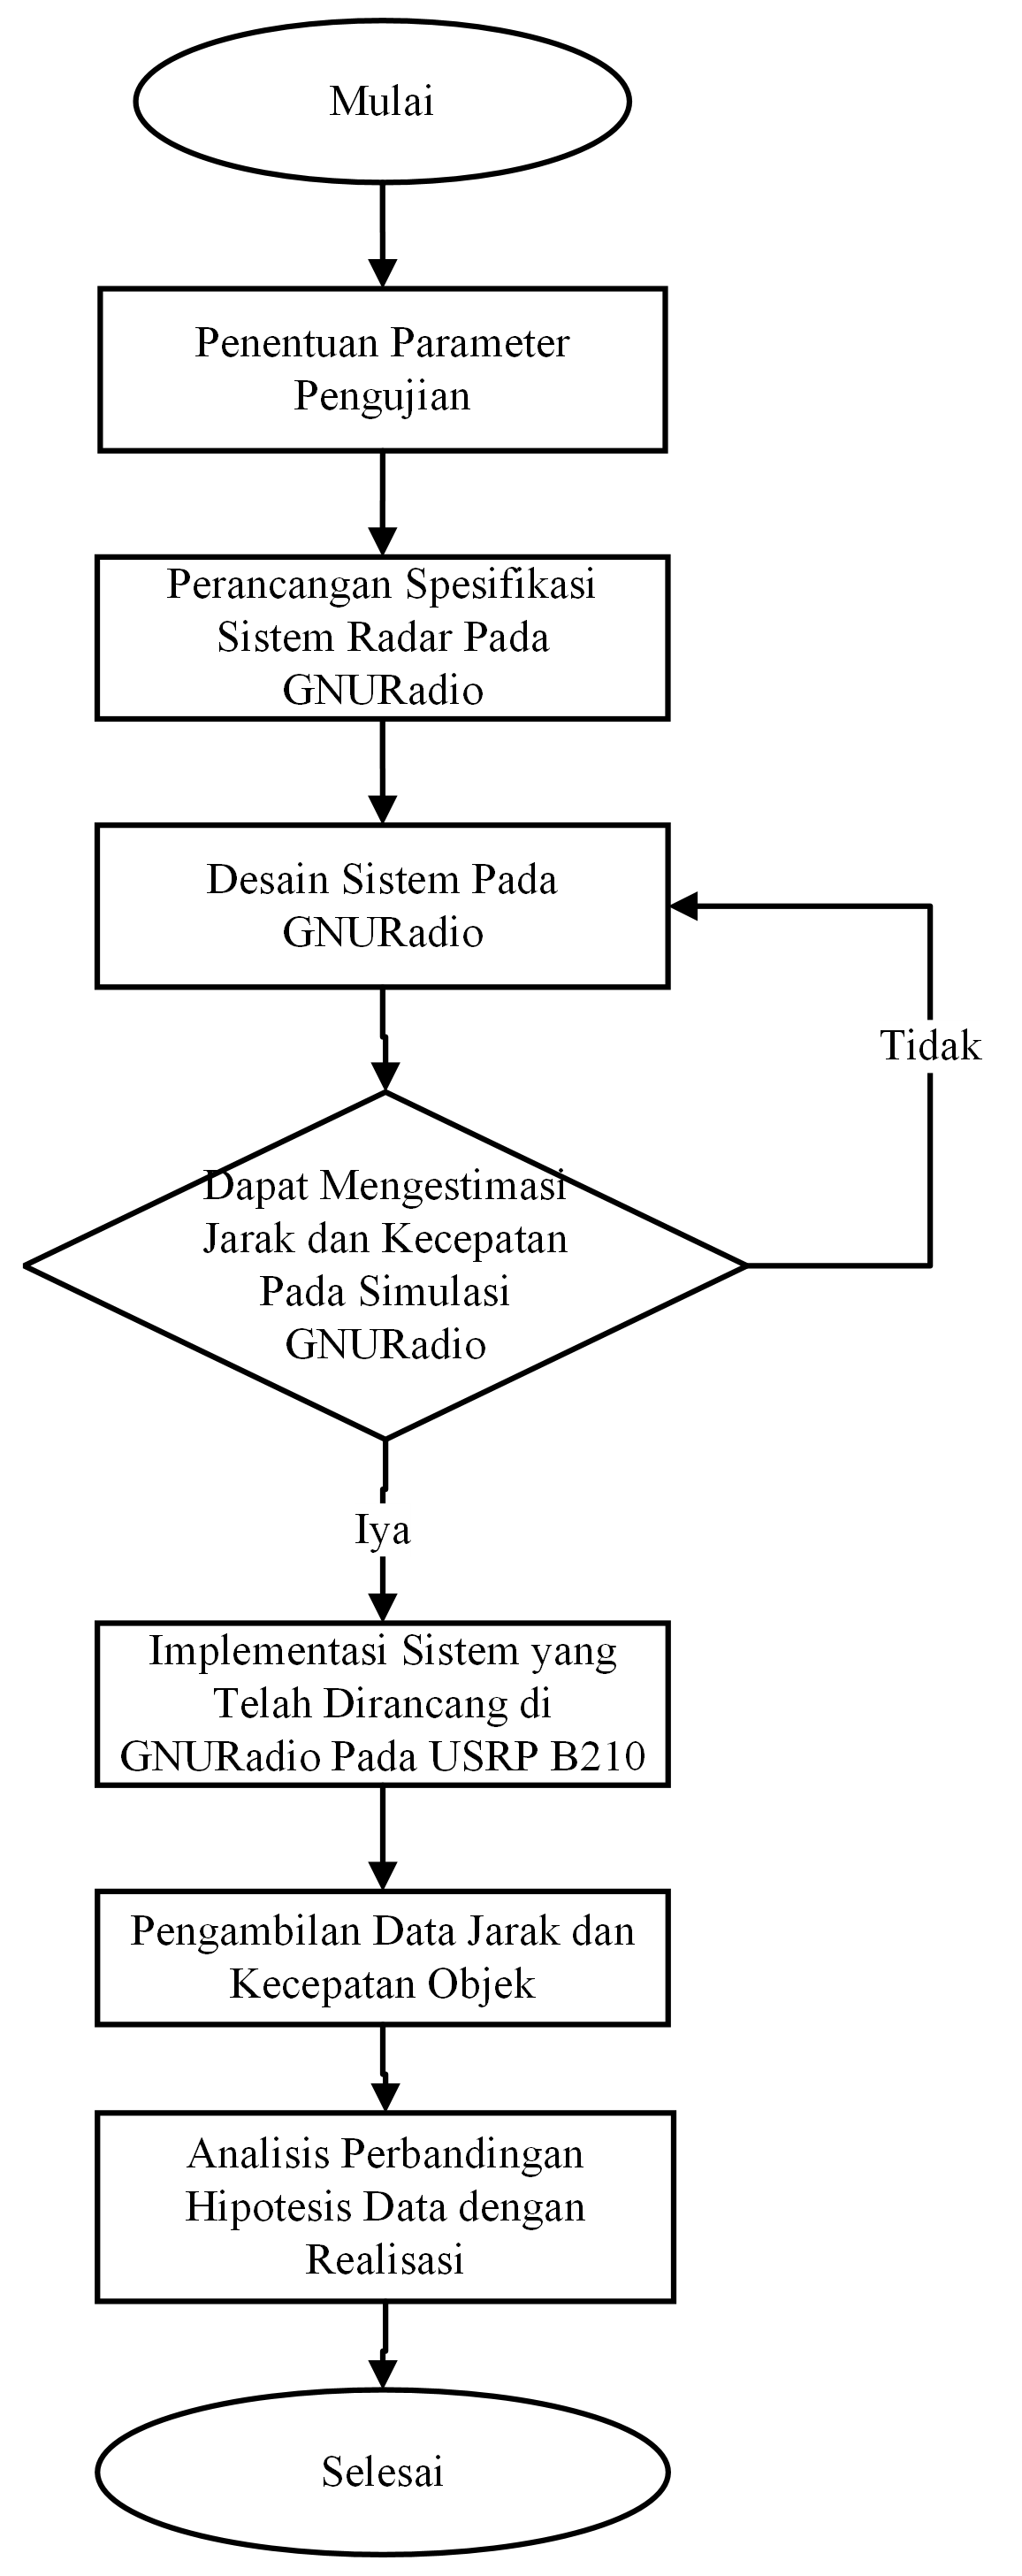
\includegraphics[scale=0.53]{pics/bab3/FlowchartTugasAkhir.png} 
		\label{img:flowchart}
		\caption[\textit{Flowchart} Penelitian]{\textit{Flowchart} Penelitian}
	\end{center}
\end{figure}
Pada alur penelitian yang telah dirancang, terdapat beberapa tahap yang perlu dilakukan setelah penelitian dimulai dan sebelum penelitian diakhiri. Tiap tahapan yang telah dirancang harus dilaksanakan sebaik mungkin agar hasil yang diharapkan dapat tercapai.
	
\section{Penentuan Parameter}

Pada tahap ini parameter pengujian ditentukan sehingga hasil yang dicapai dapat dikatakan baik, sebagai berikut.

\begin{center}
	\begin{longtable}{| c | c | c |}
		\caption{Parameter Pengujian}
		\label{tab:paramUji}\\
		\hline
		No. & Parameter Pengujian		& Satuan\\ \hline
		1.  &Jarak	   					& m\\
		2.  &Kecepatan 					& m/s\\
		3.  &\textit{RMSE}				& -\\
		4.	&Nilai prediksi \textit{beat frequency}	& Hz \\
		5.	&Nilai prediksi \textit{doppler frequency shift} & Hz \\
		\hline
	\end{longtable}
\end{center}

\section{Perancangan Spesifikasi Sistem}
Pada tahap ini, dilakukan perancangan sistem radar. Maka perlu ditentukannya spesifikasi radar berdasarkan perangkat keras USRP berseri B210 yang digunakan.  Spesifikasi dari sistem ini akan dijelaskan pada tabel berikut.

\begin{center}
	\begin{longtable}{| c | c | c |}
		\caption{Spesifikasi Sistem Radar}
		\label{tab:spekRadar}\\
		\hline
		No. & Spesifikasi 								& Keterangan\\\hline
		1.  & USRP 										& B210\\
		2.  & \textit{Carrier Frequency} ($F_{c}$) 		& 3100 MHz \\
		3.  & \textit{Bandwidth} 	(BW)				& 50 MHz \\
		4.	& Frekuensi \textit{Sampling}	($F_{s}$)	& 30 MHz	\\
		5.	& Bentuk Modulasi							& \textit{Triangular}\\
		6.  & Jarak Maksimum 		($R_{max}$)			& 145.16 km \\
		7.  & Resolusi Jarak 		($R_{res}$)			& 3 m \\
		8.  & Kecepatan Maksimum	($V_{max}$)			& 15 $m/s$ \\
		9.  & Resolusi Kecepatan 	($V_{res}$)			& 1 $m/s$\\
		10.	& Durasi \textit{Chirp}	($T_{c}$)			& 1613 $\mu s$\\
		11.	& \textit{Chirp Rate}	($\mu$)				& 0.031 $MHz/\mu s$\\
		12. & Durasi \textit{frame}	($T_{f}$)			& 48 ms \\
		\hline
	\end{longtable}
\end{center}

\begin{itemize}
	\item Hitung panjang gelombang ($\lambda$) dari frekuensi pembawa yang sudah ditentukan yaitu 3.1 GHz.
	\begin{align*}
		\lambda &= \frac{c}{F_{c}}\\
		\lambda &= \frac{3 \cdot 10^{8}}{3.1 \cdot 10^{9}}\\
		\lambda &= 0.0967 m
	\end{align*}

	\item Menghitung resolusi jarak berdasarkan persamaan \ref{eq:RangeRes} dan dengan menentukan \textit{bandwidth} bernilai 50 MHz, maka.
		\begin{align*}
			R_{res} &= \frac{c}{2 BW} \\
			R_{res} &= \frac{3 \cdot 10^{8}}{2 \cdot 50}\\
			R_{res} &= 3 m
		\end{align*}
	\item Menghitung jarak maksimum yang dapat dideteksi oleh radar digunakanlah persamaan \ref{eq:MaxRange}, namun sebelumnya harus ditentukan terlebih dahulu nilai $\mu$, yang merupakan tingkat kenaikan frekuensi pada suatu periode sesuai dengan persamaan \ref{eq:chirpRate}, dengan nilai $T_{c}$ sesuai persamaan \ref{eq:chirpTime} dan nilai kecepatan maksimum ditentukan bernilai 15 m/s, maka.
	
	\begin{align*}
		T_{c} &= \frac{\lambda}{4 \cdot V_{max}}\\
		T_{c} &= \frac{0.0967}{4 \cdot 15}\\
		T_{c} &= 1613 \mu s
	\end{align*}

	\item 
	Sehingga nilai \textit{chirp rate} ($\mu$) dapat dihitung menjadi.

		\begin{align*}
		\mu &= \frac{\textit{Bandwidth}}{T_{c}}\\
		\mu &= \frac{\textit{50}}{1613}\\
		\mu &= 0.031 MHz/ \mu s
		\end{align*}

	\item 	
	Dengan jarak maksimum yang didapat adalah.
		\begin{align*}
		R_{max} &= \frac{F_{s} \cdot c}{2 \cdot \mu}\\
		R_{max} &= \frac{30 \cdot 10^{6} \cdot 3 \cdot 10^{8}}{2 \cdot 0.031}\\
		R_{max} &= 145.16 km
		\end{align*}

	\item 
	Dengan $T_{f}$ sebagai durasi \textit{frame} bernilai 0.048 s maka resolusi kecepatannya.
		\begin{align*}
			V_{res} &= \frac{\lambda}{2 \cdot T_{f}}\\
			V_{res} &= \frac{0.0967}{2 \cdot 0.048}\\
			V_{res} &= 1 m/s
		\end{align*}

\end{itemize}

\section{Implementasi Sistem}
Tahap implementasi ini dilakukan pada aplikasi GNURadio dan menghasilkan \textit{flow diagram} yang merepresentasikan langkah yang dilakukan pada USRP. \textit{Flow diagram} yang didesain sudah memenuhi spesifikasi sistem radar pada tabel \ref{tab:spekRadar}. 

Implementasi sistem akan dilaksanakan pada beberapa perangkat, mulai dari laptop, antena, dan USRP. Berikut detail perangkat yang akan digunakan pada saat implementasi guna mendapat hasil yang baik.

\begin{enumerate}
	\item \textit{IdeaPad Gaming 3 15ARH7} :
	\begin{figure}
		\begin{center}
			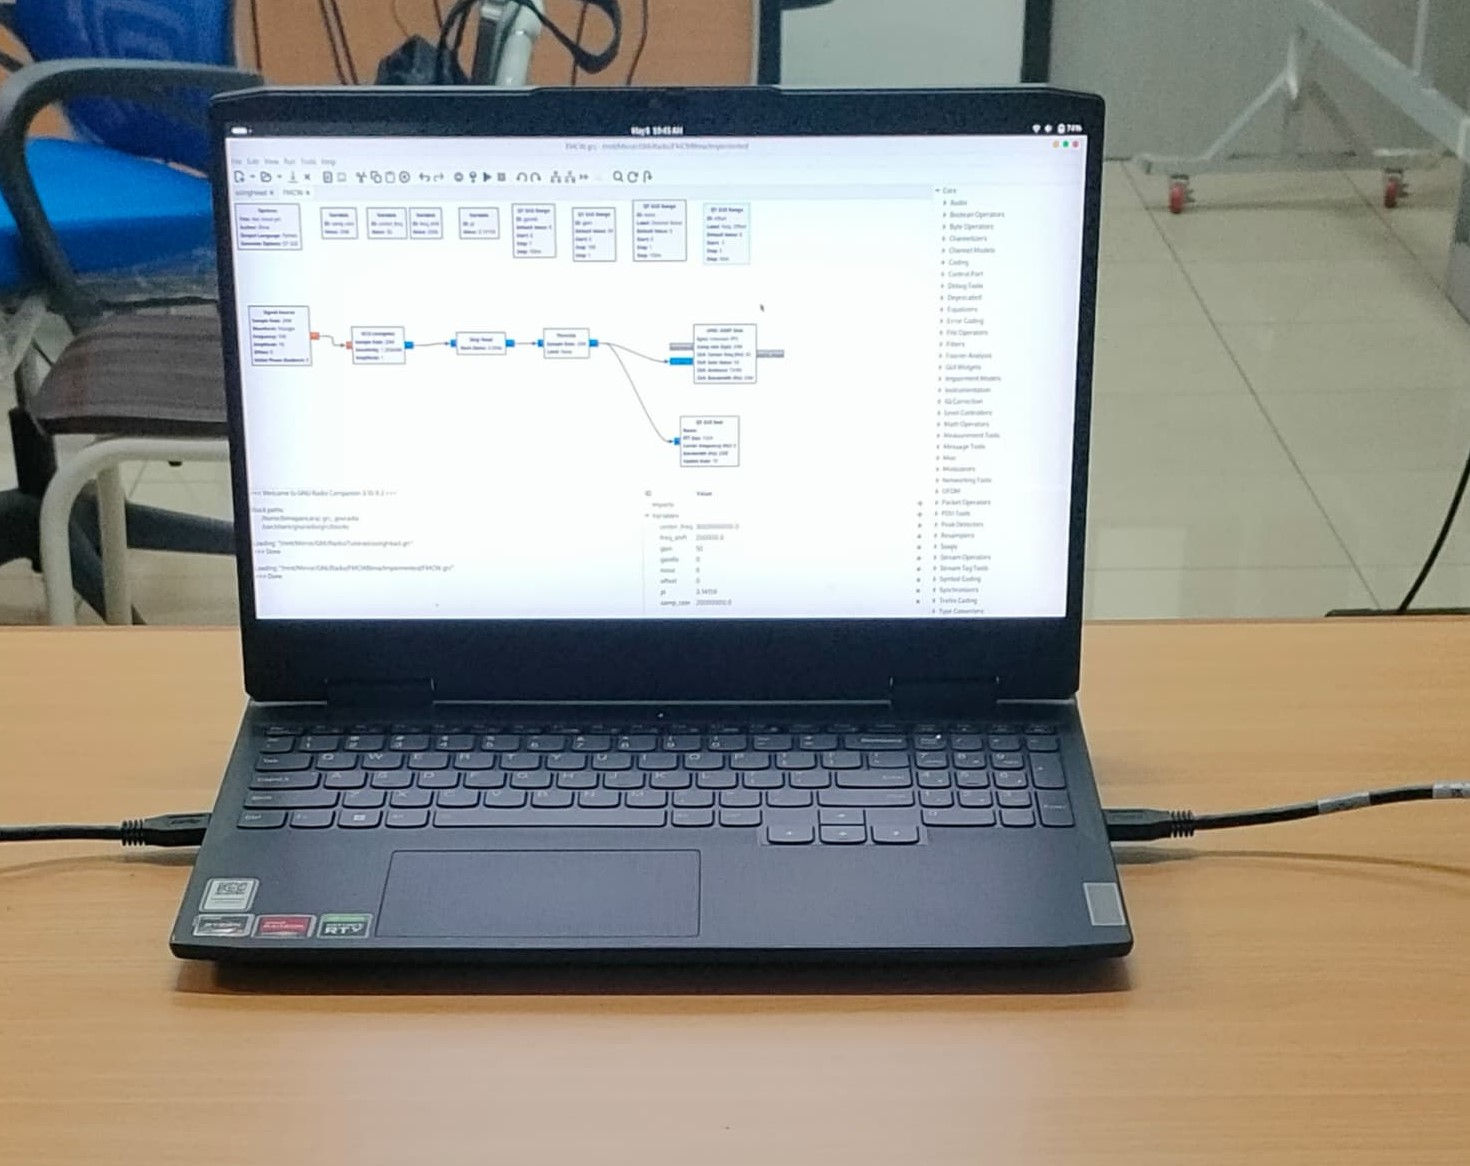
\includegraphics[scale=0.2]{pics/bab3/laptop.jpg} 
			\caption[Gambar Perangkat Laptop Yang Digunakan]{Gambar Perangkat Laptop Yang Digunakan}
			\label{pic:contohBlokGRC}
		\end{center}
	\end{figure}

	\begin{itemize}
		\item \textit{Processor} : AMD Ryzen 7 6800H dengan \textit{Radeon Graphics} 3.20 GHz
		\item \textit{Memory} : 8,00 GB (7,19 GB \textit{usable})
	\end{itemize}

	\item Perangkat \textit{Software Defined Radio} :
	\begin{figure}
		\begin{center}
			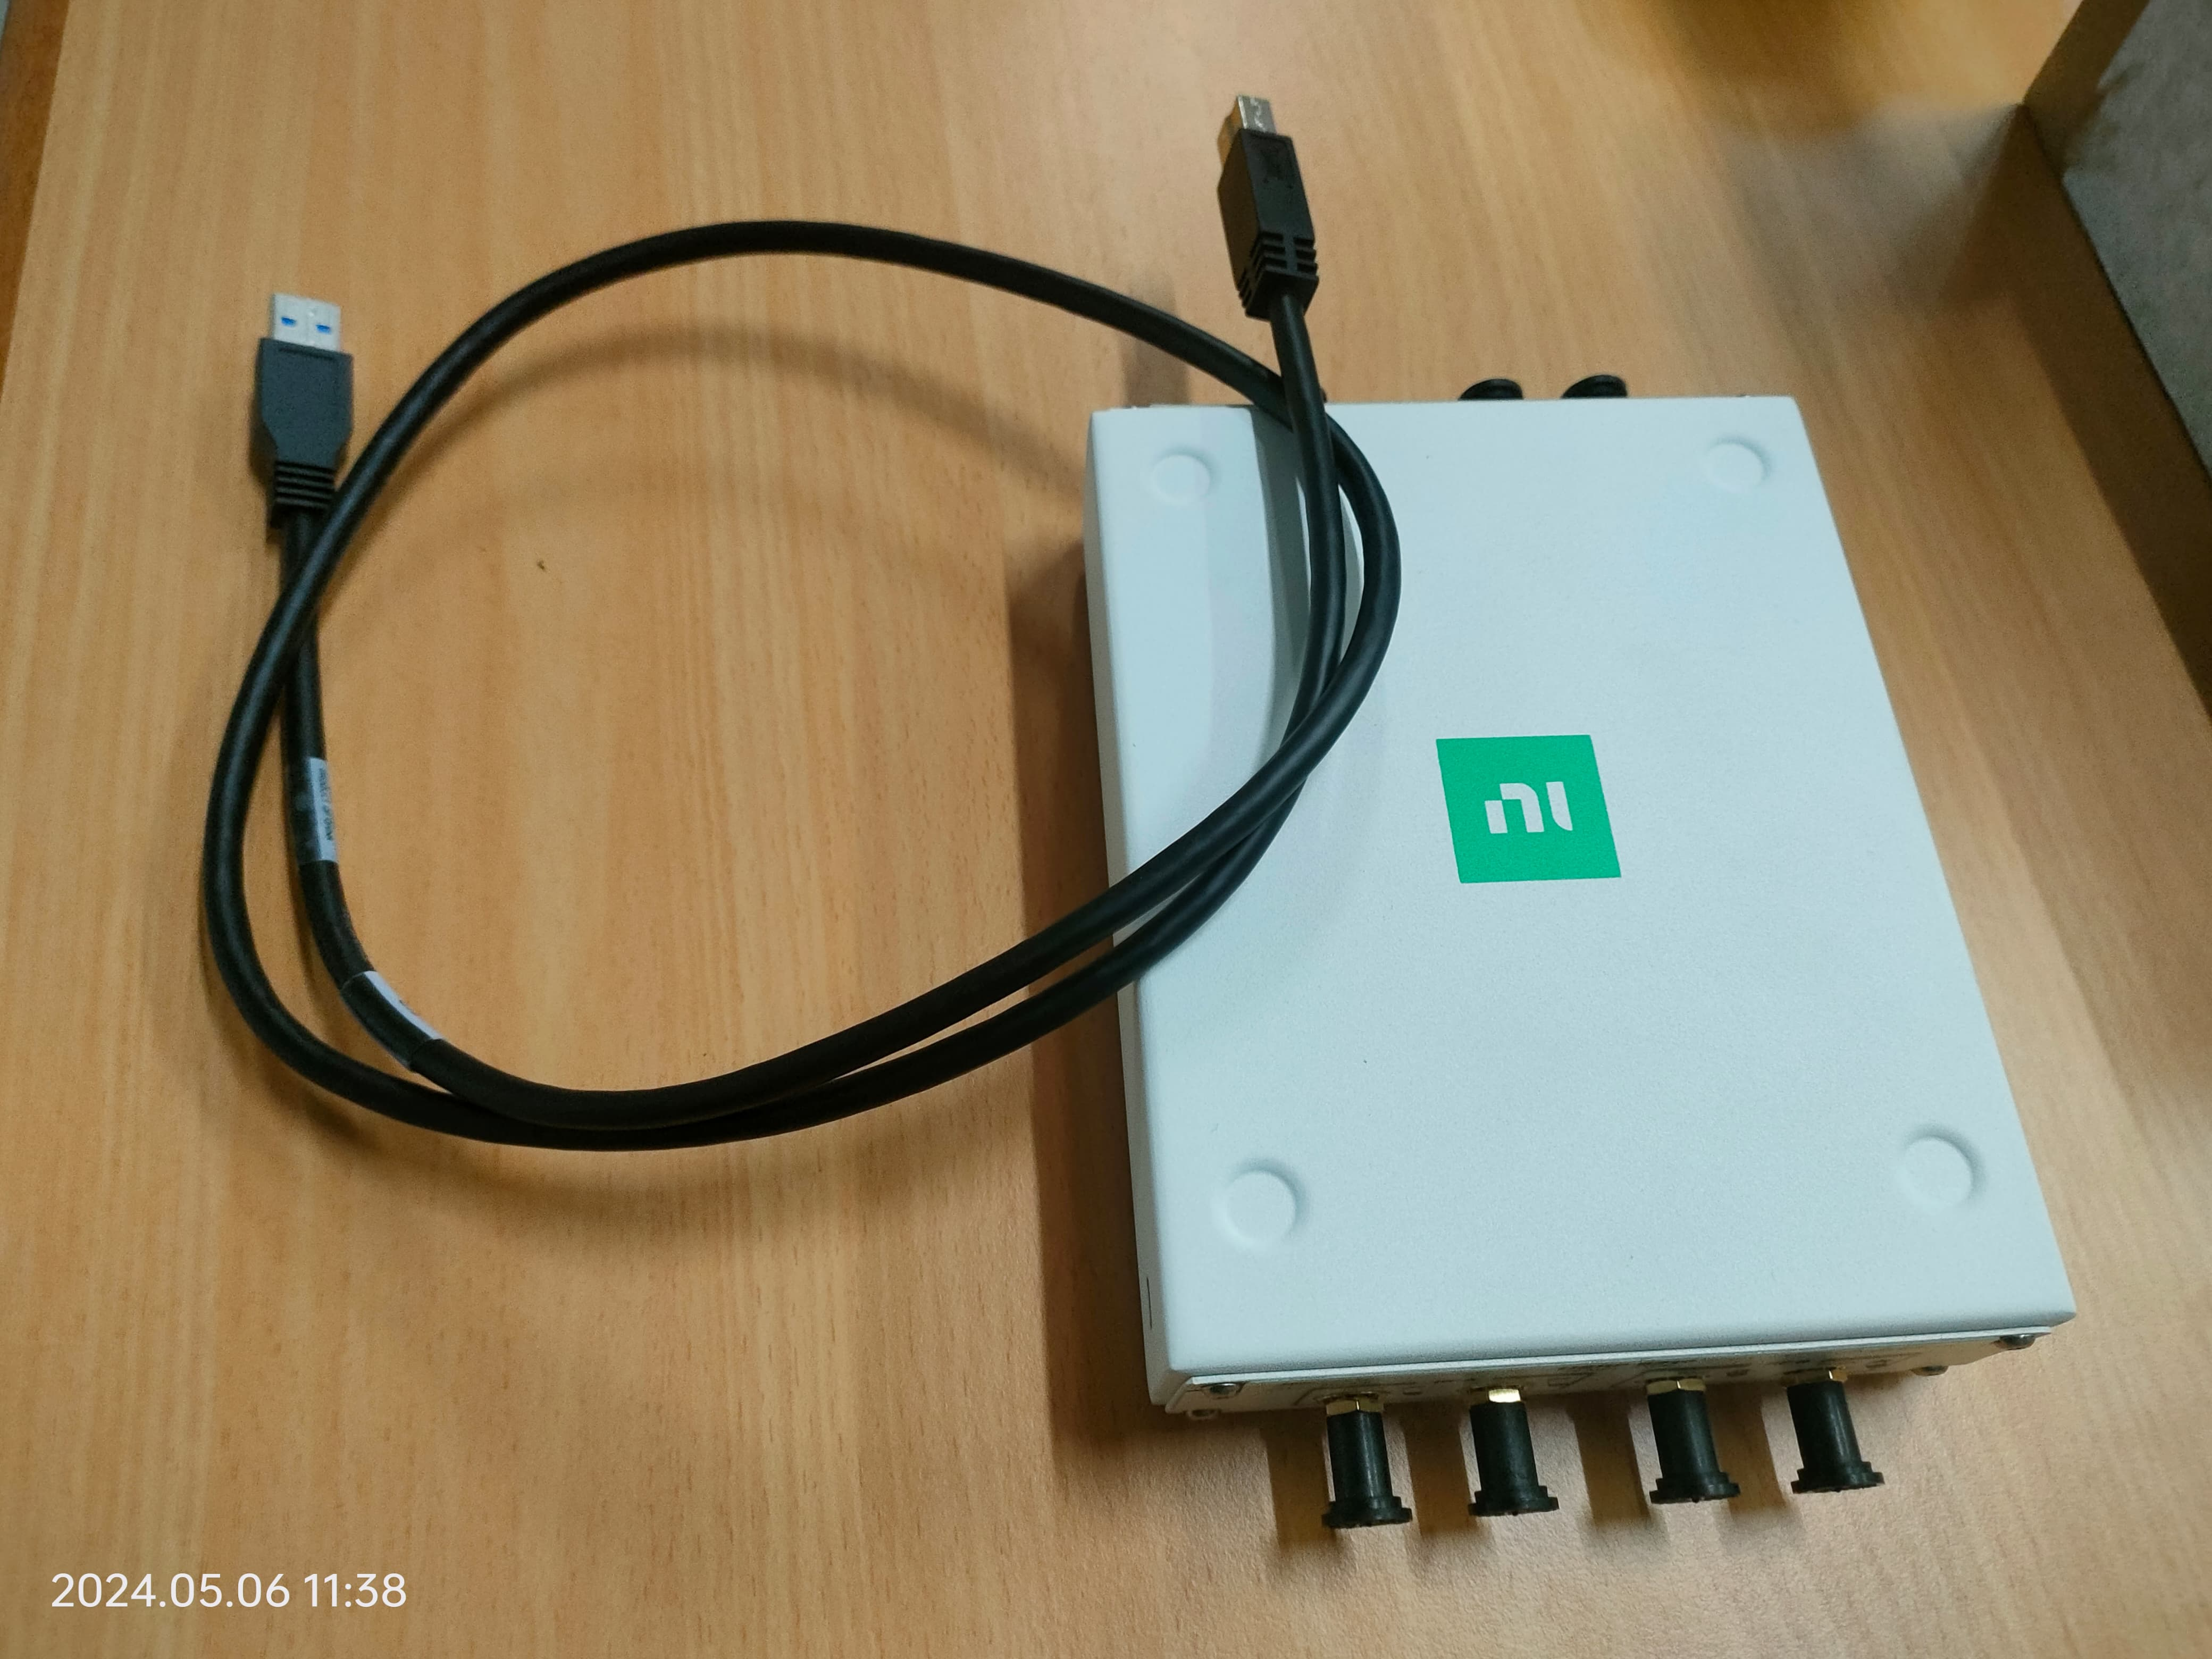
\includegraphics[scale=0.045]{pics/bab3/usrp2.jpg}
			\caption{Alat USRP B210}
			\label{img:logPeriodic}
		\end{center}
	\end{figure}
	\begin{itemize}
		\item Tipe : USRP B210 
		\item Jarak Frekuensi : 70 MHz - 6000 MHz 
	\end{itemize}

	\item Antena \textit{Log-periodic} :
	\begin{figure}
		\begin{center}
			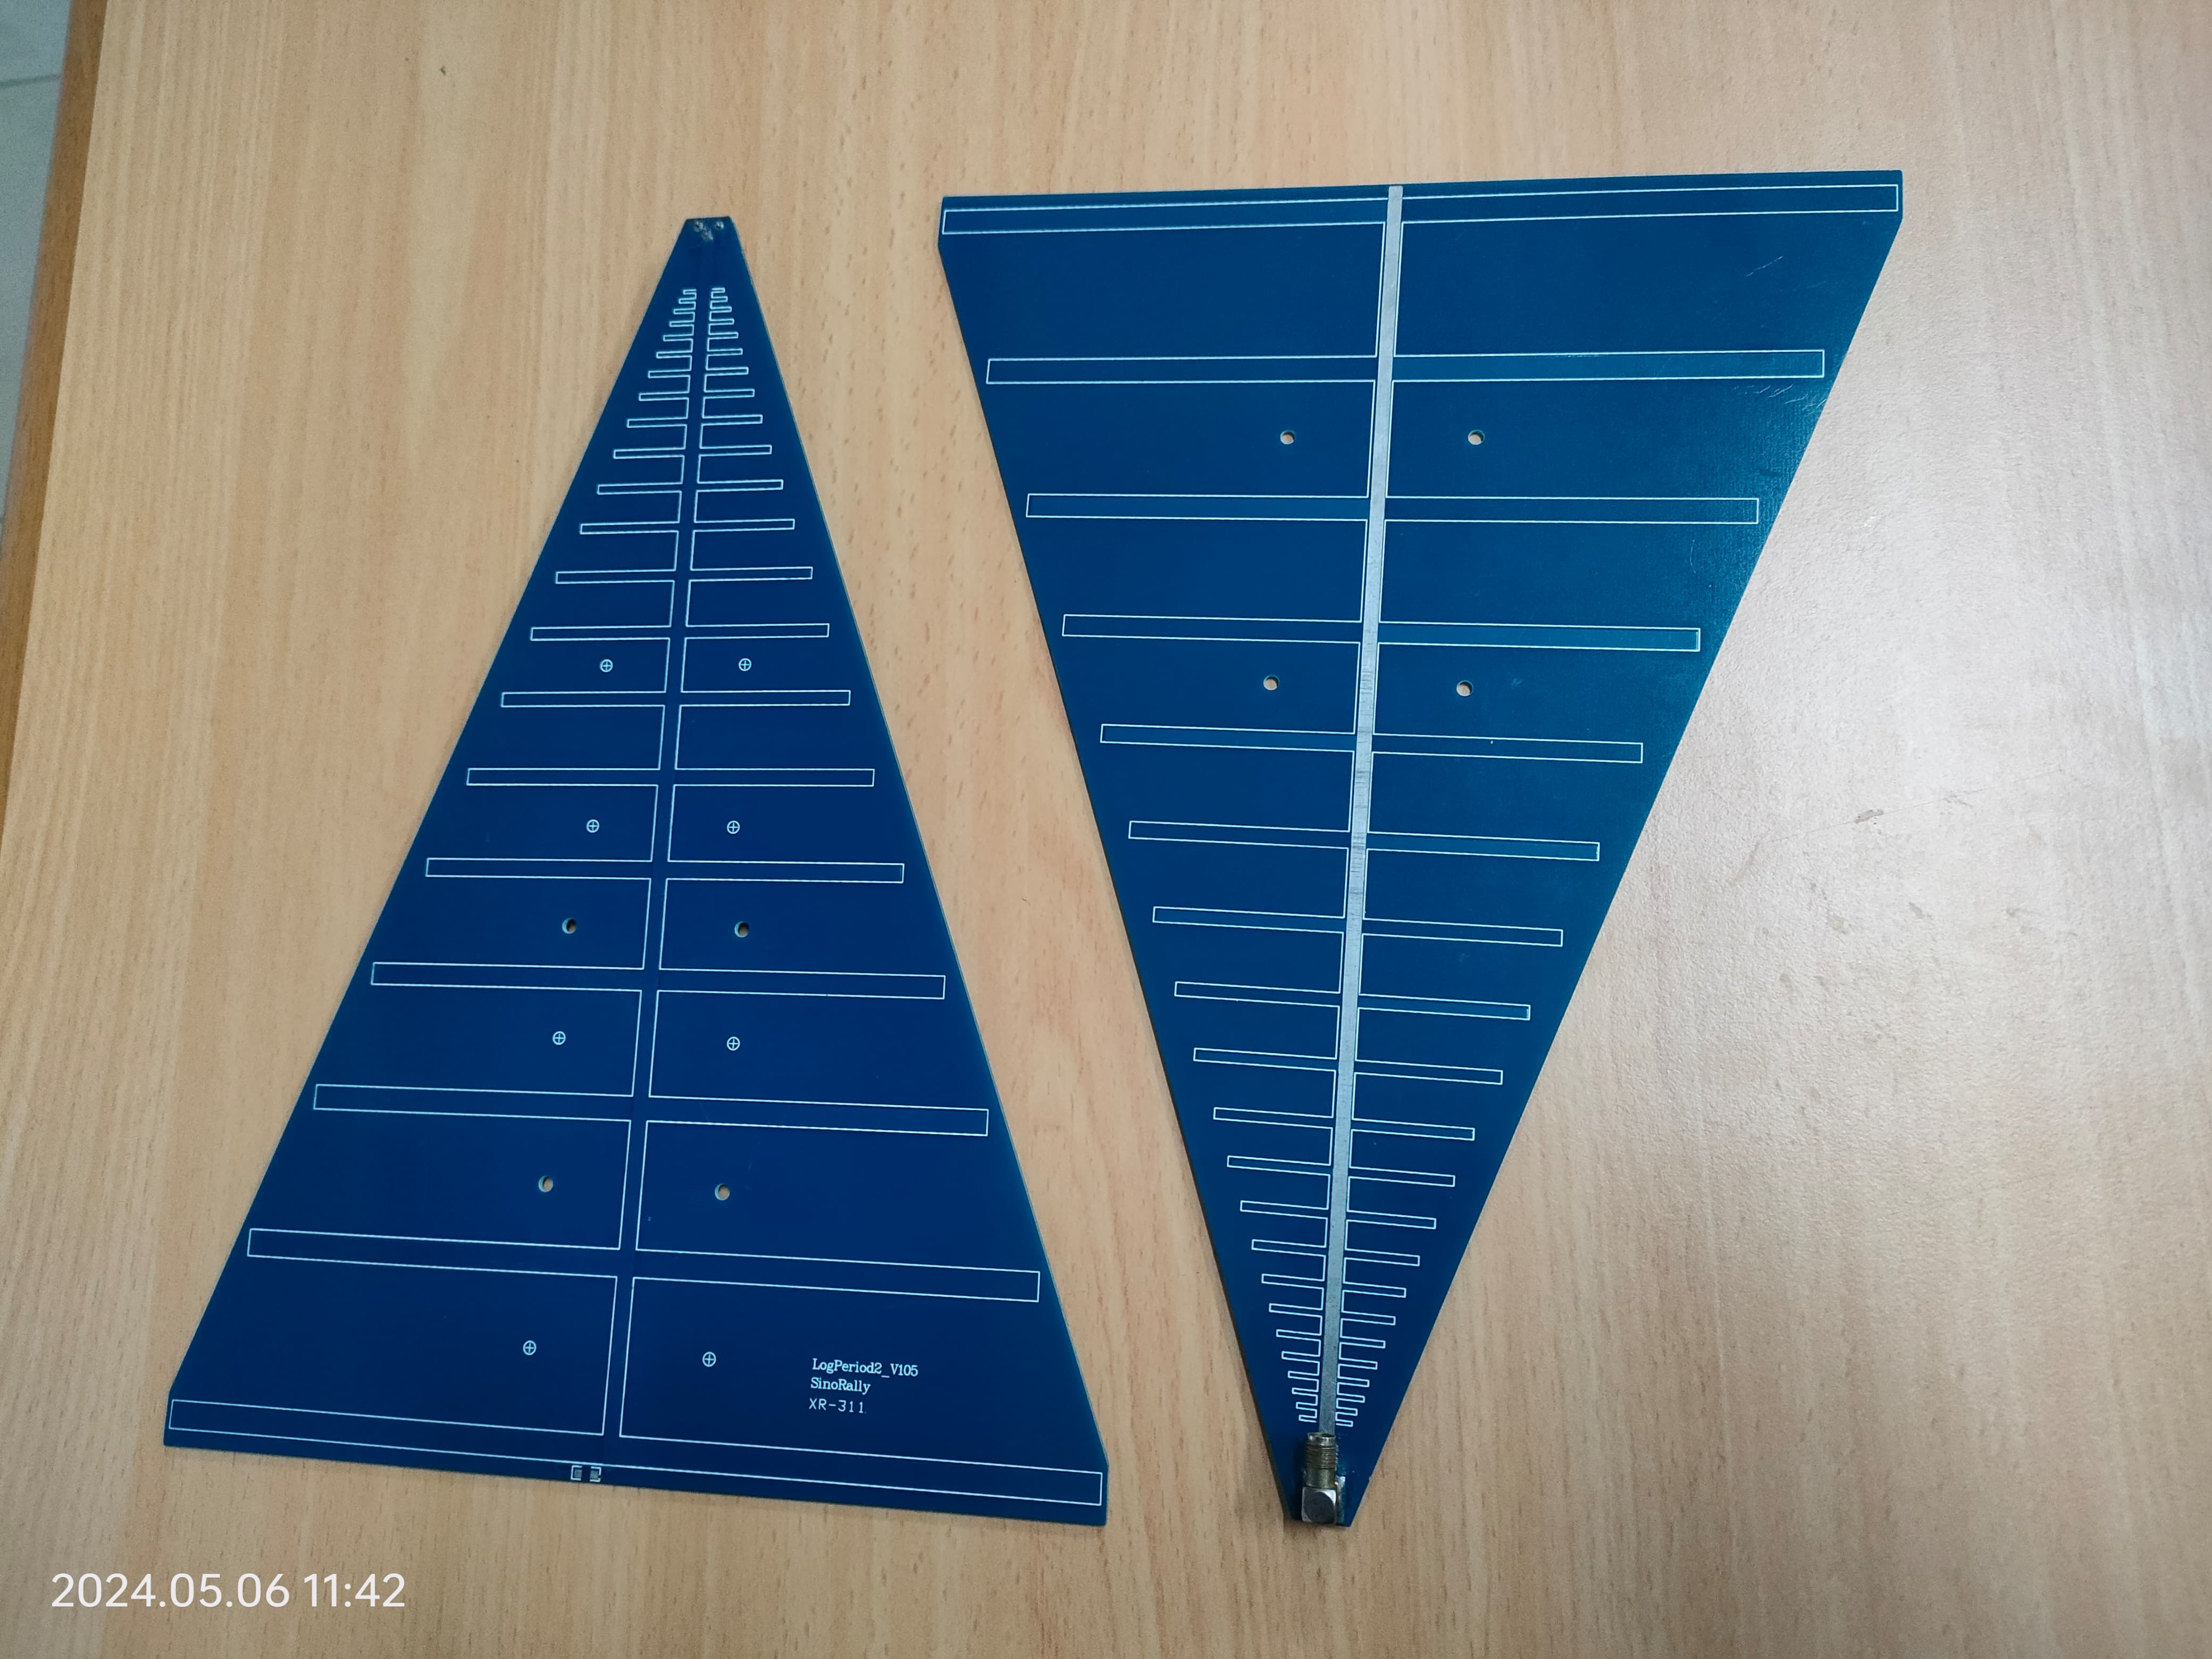
\includegraphics[scale=0.05]{pics/bab3/logPeriodic.jpg}
			\caption{Antena \textit{Log Periodic} Pengujian}
			\label{img:usrpBoard}
		\end{center}
	\end{figure}
	\begin{itemize}
		\item Frekuensi : 800 MHz - 6000 MHz 
		\item Pola Radiasi : \textit{Directional}
		\item \textit{Gain} : 5.2 - 6.3 dB
	\end{itemize}
\end{enumerate}

	
\section{Pengambilan Data}
Pada tahap ini, pengambilan data dengan radar yang sudah didesain dan diimplementasikan pada USRP dilakukan. Pengujian dilakukan dengan menggunakan kendaraan roda empat sebagai objek yang akan dideteksi. Sehingga pengambilan data kecepatan dan prediksi jarak dapat dilakukan. Hasil prediksi jarak dan kecepatan radar akan dibandingkan dengan nilai aktual jarak pada kenyataan dan kecepatan tercatat pada \textit{speedometer}.

\begin{figure}
	\begin{center}
		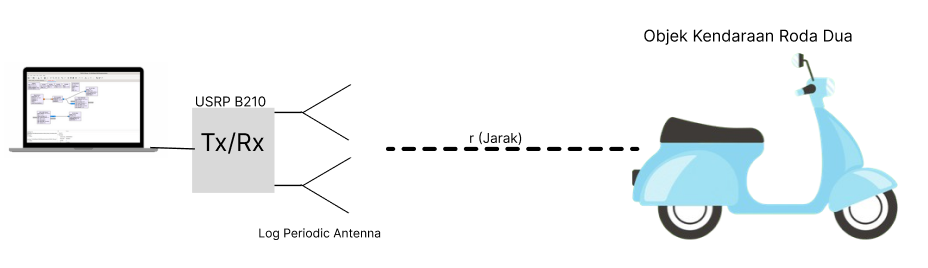
\includegraphics[scale=0.55]{pics/bab3/skema.png}
		\caption{Skema Penelitian}
		\label{img:skema}
	\end{center}
\end{figure}

Data berupa nilai \textit{beat frequency} dan \textit{doppler frequency shift} yang sudah ditentukan sebagai parameter pengujian telah didapat dari hasil pengambilan data akan dibandingkan dengan nilai prediksi berdasarkan perhitungan. Dengan begitu, maka nilai RMSE dapat dihitung.

\begin{figure}
	\begin{center}
		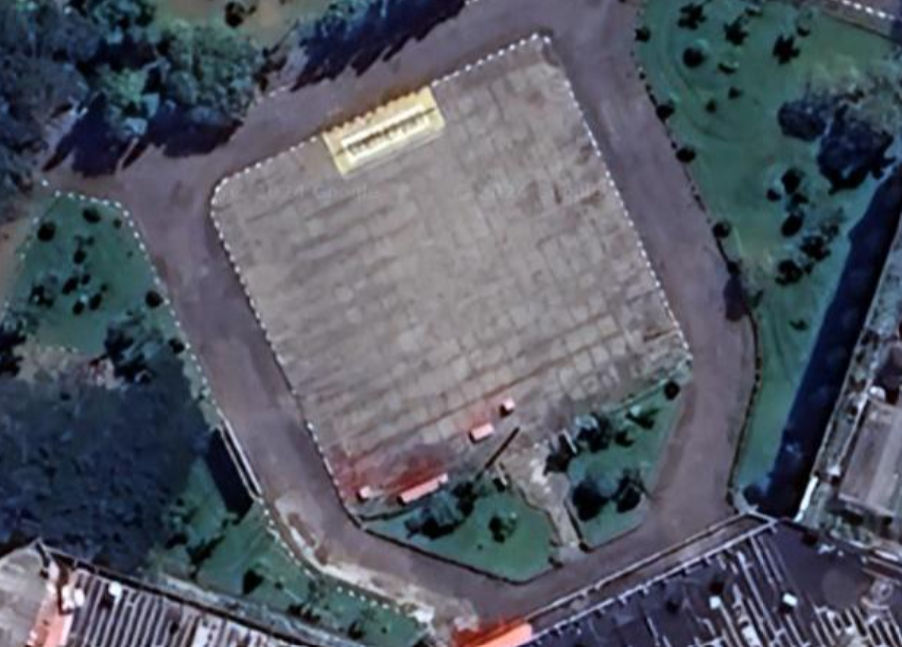
\includegraphics[scale=0.35]{pics/bab3/petaPengujian.png}
		\caption{Lokasi Pengujian}
		\label{img:petaUji}
	\end{center}
\end{figure}

Pengambilan data akan dilaksanakan di lokasi lapangan Universitas Telkom Surabaya yang beralamat Jl. Ketintang No.156, Ketintang, Kec. Gayungan, Surabaya, Jawa Timur 60231.

\section{Konfigurasi Pengujian}
Konfigurasi pengujian dilakukan sesuai dengan gambar \ref{img:skema}. Terdapat satu buah perangkat laptop yang terhubung dengan dua buah USRP, masing-masing USRP terhubung dengan antena \textit{Log-periodic}. USRP 1 berperan sebagai \textit{transmitter} sedangkan USRP 2 berperan sebagai \textit{receiver}.

\begin{figure}
	\begin{center}
		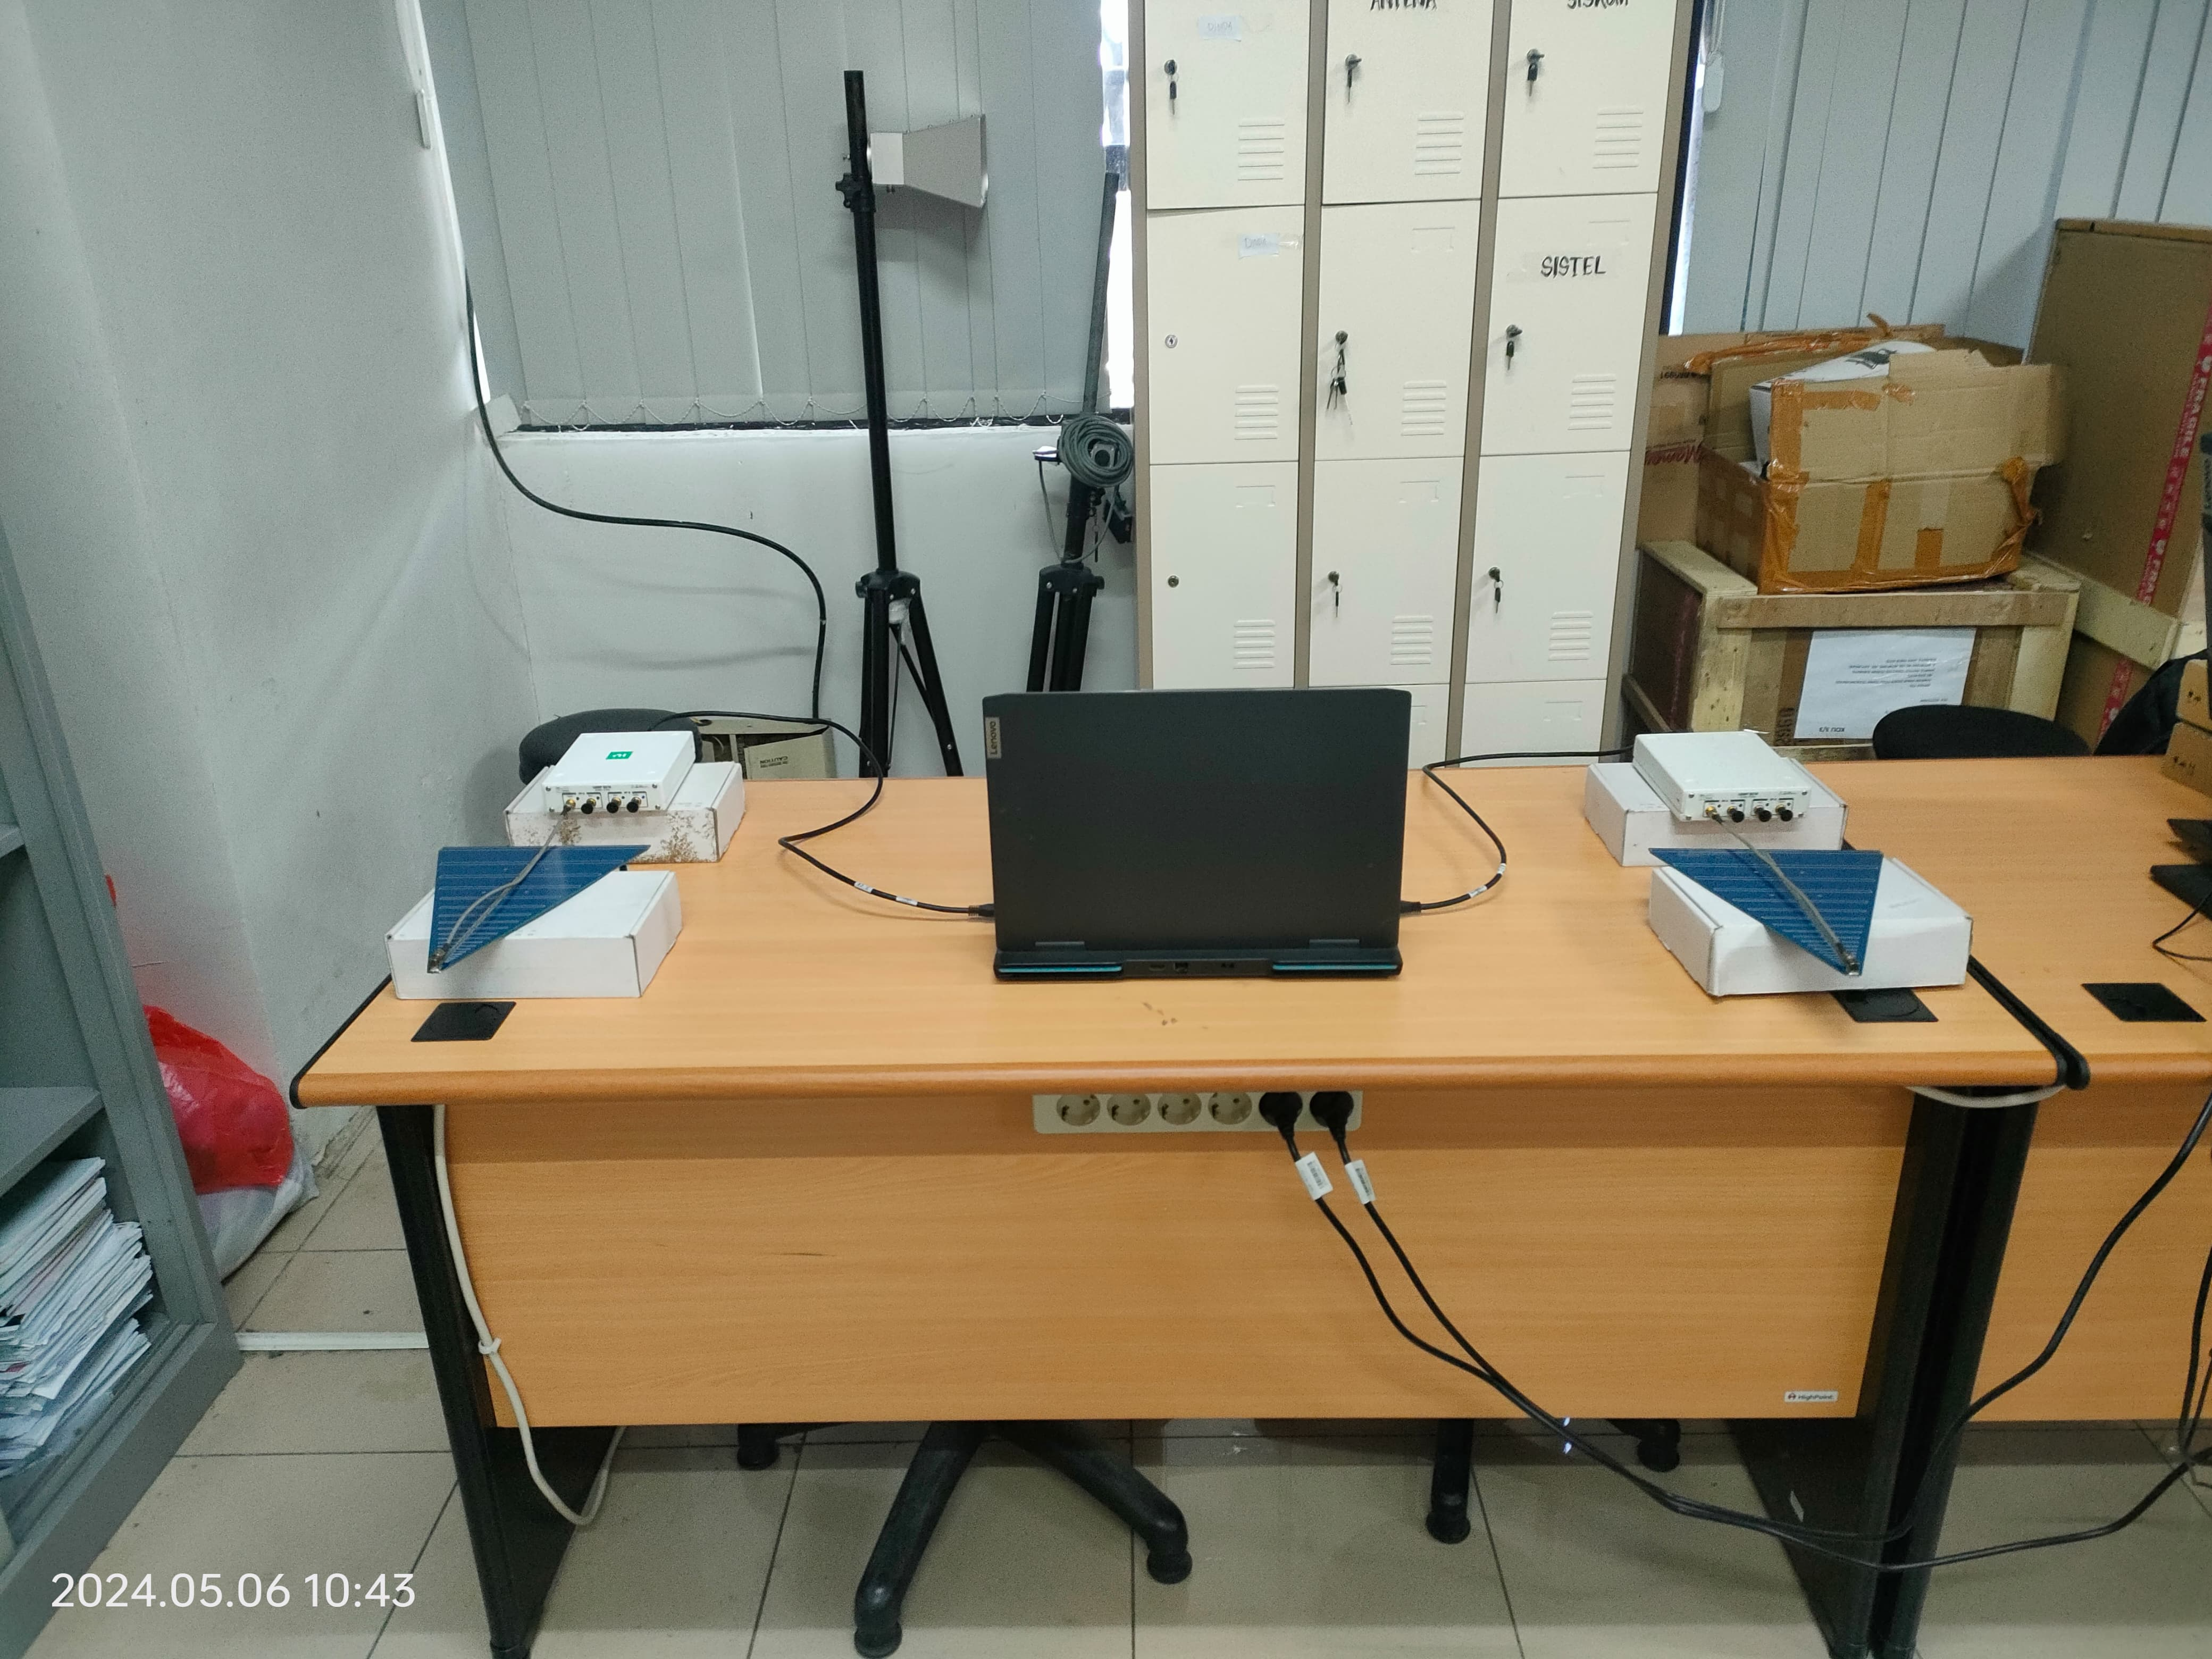
\includegraphics[scale=0.09]{pics/bab3/konfigurasiPengujian.jpg}
		\caption{Konfigurasi Pengujian}
		\label{img:konfigurasi}
	\end{center}
\end{figure}


\section{Prediksi Hasil Pengujian}

Prediksi hasil pengujian diperlukan untuk menjadi pembanding dari hasil yang akan didapat setelah melakukan pengujian. Perhitungan prediksi ini berupa nilai \textit{beat frequency} dan \textit{doppler frequency}. Prediksi nilai \textit{beat frequency} didapat pada persamaan \ref{eq:RangeEst} dan memodifikasinya dengan menentukan nilai jarak ($d_{0}$) pada estimasi jarak. Sehingga akan didapat persamaan estimasi \textit{beat frequency}($f_{b}$) seperti berikut.

\begin{equation}
	f_{b} = \frac{d_{0} \cdot 2 \mu}{c} = \frac{d_{0} \cdot 2BW}{c \cdot T_{c}}
	\label{eq:predFb}
\end{equation}

Persamaan \ref{eq:predFb} menunjukkan bahwa dengan menentukan jarak ($d_{0}$) dalam meter, \textit{chirp rate} ($\mu$) dalam $Hz/\mu s$, kecepatan cahaya (c) dalam $m/s$, lebar pita frekuensi (BW) dalam Hz, dan waktu \textit{chirp} ($T_{c}$) dalam $\mu s$. Maka \textit{beat frequency} ($f_{b}$) yang ditemukan akan memiliki satuan Hz.


Prediksi nilai frekuensi doppler dapat dilakukan dengan mengubah persamaan \ref{eq:velocity} lalu memberikan asumsi nilai kecepatan (v) pada estimasi kecepatan dengan satuan m/s dan panjang gelombang frekuensi ($\lambda$) yang digunakan dengan satuan meter. Sehingga persamaan estimasi \textit{doppler frequency} ($f_{d}$) akan menjadi berikut.

\begin{equation}
	f_{d} = \frac{v \cdot 2}{\lambda}
	\label{eq:predFd}
\end{equation}

Hasil prediksi dari nilai \textit{beat frequency} yang telah dihitung menggunakan persamaan \ref{eq:predFb} berada pada tabel \ref{tab:predFbeat}.

\begin{center}
	\begin{longtable}{|c|c|}
		\caption{Prediksi Nilai \textit{Beat Frequency}}
		\label{tab:predFbeat}\\
		\hline
		d0 & Prediksi $f_{b}$  \\
		\hline
		5 m & 1033 Hz\\
		\hline
		10 m & 2067 Hz\\
		\hline
		15 m & 3100 Hz\\
		\hline
		20 m & 4133 Hz\\
		\hline
		25 m & 5167 Hz\\
		\hline
	\end{longtable}
\end{center}

Hasil prediksi dari nilai \textit{doppler frequency} yang didapat dengan persamaan \ref{eq:predFd} terdata dalam tabel \ref{tab:predFdopp}.

\begin{center}
	\begin{longtable}{|c|c|}
		\caption{Prediksi Nilai \textit{Doppler Frequency}}
		\label{tab:predFdopp}\\
		\hline
		v & Prediksi $f_{d}$  \\
		\hline
		3 m & 62 Hz\\
		\hline
		6 m & 124 Hz\\
		\hline
		9 m & 186 Hz\\
		\hline
		12 m & 248 Hz\\
		\hline
		15 m & 310 Hz\\
		\hline
	\end{longtable}
\end{center}